%\documentclass[12pt,handout]{beamer}
%\documentclass{beamer}
\usepackage[ngerman]{babel}
\usepackage[utf8]{inputenc}
\usepackage{amsmath}
\usepackage{amssymb}
\usepackage{listings} 
\usepackage{stmaryrd}
\lstset{language=Python, tabsize=4, showstringspaces=false,basicstyle=\scriptsize,mathescape=true}  
\lstset{literate=%
  {Ö}{{\"O}}1
  {Ä}{{\"A}}1
  {Ü}{{\"U}}1
  {ß}{{\ss}}1
  {ü}{{\"u}}1
  {ä}{{\"a}}1
  {ö}{{\"o}}1
}
\usepackage{mathtools}
\usepackage{ulem}
\usepackage{tikz}

\usetheme{Boadilla}
\mode<presentation>{
\useoutertheme[subsection=false]{miniframes}
\useinnertheme{rectangles}
%\usecolortheme{crane}
}
\parskip 10pt



\begin{document}
\title{Informatik}   
\author{Suchalgorithmen am Beispiel 8-Puzzle} 
\date{}
\frame{\titlepage} 

%---
\begin{frame}[fragile]

In vielen Problemstellung geht es darum, in einer (meist sehr großen) Menge von Möglichkeiten eine Lösung zu finden. 
Am Beispiel des 8-Puzzle werden verschiedene Suchalgorithmen für das Finden einer Lösung vorgestellt.


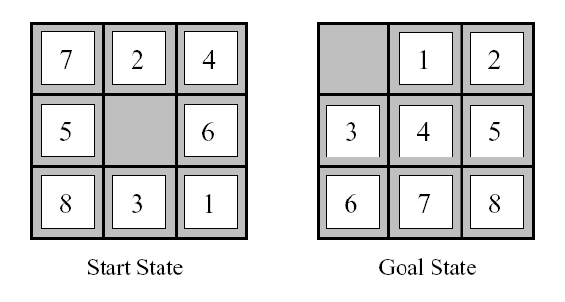
\includegraphics[scale=0.6]{bild1.png}

\url{http://mypuzzle.org/sliding}

\end{frame}

\begin{frame}[fragile]
Einzelne Spielstellungen stellen wir uns als Knoten vor. Die Kanten zwischen den Knoten sind mögliche Spielzüge.
Die Startstellung ist also die Wurzel eines Suchbaums, in dem wir einen Pfad zu einem Knoten suchen, der den \texttt{goaltest} besteht. 

In der Regel ist der Suchbaum so groß, dass er nicht in seiner Gesamtheit aufgebaut werden kann. Während der Suche wird der Suchbaums immer wieder erweitert und wir hoffen, dass wir auf eine Lösung stoßen, ohne den gesamten Baum durchsuchen zu müssen.
\end{frame}

\begin{frame}[fragile]
Die Knoten, die wir noch untersuchen müssen, verwalten wir in der \texttt{frontier} (fringe, open set).
Zu jedem Knoten, der in die \texttt{frontier} kommt, merken wir uns den Elternknoten in einem dictionary \texttt{prev}.
Zu Beginn ist nur der Startknoten in der \texttt{frontier} mit Elternknoten \texttt{None}.

Wenn wir einen Knoten untersuche, holen wir ihn aus der \texttt{frontier} und schauen, ob er den \texttt{goaltest} besteht.
Wenn das nicht der Fall ist, gehen wir die Liste seiner Kinder durch. Nur Kinder, die noch nicht key im dictionary \texttt{prev} sind, werden der \texttt{frontier} hinzugefügt.

\end{frame}


\begin{frame}[fragile]
\small
Wir gehen davon aus, dass wir folgende Funktionen zur Verfügung haben:

\begin{lstlisting}  [basicstyle = \tiny]
def nextstates(state):
    '''
    state: Spielstellung
    returns: eine Liste oder Menge von möglichen Folgestellungen zu state
    '''

def goaltest(state):
    '''
    state: Spielstellung
    returns: True, wenn Spielstellung einen Lösung ist
    '''
\end{lstlisting} 
\small
Wenn wir bei einer Spielstellung angekommen sind, die den \texttt{goaltest} besteht, interessiert uns der Weg, wie wir dahin gekommen sind. Dazu merken wir uns für jede untersuchte Spielstellung deren Vorgänger in einem dictionary \text{prev}. Die Funktion \texttt{reconstructPath} ermittelt dann den Weg zur Lösung.

\begin{lstlisting}  [basicstyle = \tiny]
def reconstructPath(prev):
    '''
    prev: dictionary, das jeder Spielstellung ihren Vorgänger zuordnet.
       Die Startstellung hat als Vorgänger None zugeordnet.
    returns: String-Repräsentation des Weges von der Start- zur Zielstellung
    '''

\end{lstlisting} 
\end{frame}

\begin{frame}[fragile]
Breitensuche: frontier ist Queue

\begin{lstlisting} 
Initialisiere frontier als Queue mit dem startstate
Initialisiere prev als dictionary der Vorgänger
Der Vorgänger von startstate ist None

solange frontier nicht leer:
    hole state aus frontier
    
    wenn goalTest(state):
        return dictionary mit Vorgängern
    
    für jedes v aus nextstates(state):
        wenn für v kein Eintrag in prev vorhanden:
            füge v in die frontier ein.
            merke state als Vorgänger von v
    

\end{lstlisting} 
\end{frame}

\begin{frame}[fragile]
\begin{lstlisting} 
from collections import deque
def bfs(s):
    ''' 
    s: Startstellung
    returns: dictionary mit den Vorgängern der Spielstellungen
        auf dem  Weg zum Ziel, None wenn Ziel nicht gefunden
    '''   $\pause$
    frontier =  deque([s])
    prev = {s:None}
    while frontier:
        state = frontier.popleft()  
        if goaltest(state):
            return prev
        for v in nextstates(state):
            if v not in prev:
                frontier.append(v)
                prev[v] = state

\end{lstlisting} 
\end{frame}



\begin{frame}[fragile]
Eine Spielstellung modellieren wir mit einem 9-Tuple. \\
(7,2,4,5,0,6,8,3,1) entspricht der Spielstellung
\begin{lstlisting} 
7 2 4
5   6
8 3 1
\end{lstlisting} 

\begin{lstlisting} [basicstyle = \scriptsize]
def goaltest(state):
    '''
    state: Spielstellung
    returns: True, wenn state Zielposition ist
    '''  $\pause$
    return state $==$ (0,1,2,3,4,5,6,7,8) 
\end{lstlisting} 
\end{frame}

\begin{frame}[fragile]
\begin{lstlisting} [basicstyle = \scriptsize]
def swap(state,i,j):
    '''
    state: Spielstellung
    i, j: ints zwischen 0 und 8
    returns: Spielstellung, bei der gegenüber state 
       die Zahlen an den Positionen i und j vertauscht sind.
    ''' $\pause$
    temp = list(state)
    temp[i],temp[j] = temp[j],temp[i]
    return tuple(temp)
\end{lstlisting} 
\end{frame}

\begin{frame}[fragile]
\begin{lstlisting} [basicstyle = \tiny]
def nextstates(state):
    '''
    state: Spielstellung
    returns: Liste mit den möglichen Folgestellungen für state. Die möglichen Bewegung
       des Leerfeldes halten sich an die Reihenfolge: up, down, left, right 
    ''' $\pause$
    if state[0] $==$ 0:   return [swap(state,0,3),swap(state,0,1)]
    elif state[1] $==$ 0: return [swap(state,1,4),swap(state,1,0),swap(state,1,2)]
    elif state[2] $==$ 0: return [swap(state,2,5),swap(state,2,1)]
    elif state[3] $==$ 0: return [swap(state,3,0),swap(state,3,6),swap(state,3,4)]
    elif state[4] $==$ 0: return [swap(state,4,1),swap(state,4,7),swap(state,4,3)
                                ,swap(state,4,5)]
    elif state[5] $==$ 0: return [swap(state,5,2),swap(state,5,8),swap(state,5,4)]
    elif state[6] $==$ 0: return [swap(state,6,3),swap(state,6,7)]
    elif state[7] $==$ 0: return [swap(state,7,4),swap(state,7,6),swap(state,7,8)]
    elif state[8] $==$ 0: return [swap(state,8,5),swap(state,8,7)]
\end{lstlisting} 
\end{frame}

\begin{frame}[fragile]
\begin{lstlisting}  [basicstyle = \scriptsize]
def reconstructPath(prev):
    '''
    prev: dictionary, das jeder Spielstellung ihren Vorgänger 
       zuordnet. Die Startstellung hat als Vorgänger 
       None zugeordnet.
    returns: String-Repräsentation des Weges von 
       der Start- zur Zielstellung
    '''   $\pause$
    s = (0,1,2,3,4,5,6,7,8)
    tmp = []
    while prev[s] is not None:
        i = s.index(0)
        ip = prev[s].index(0)
        if i $==$ ip-1: tmp.append('left')
        elif i $==$ ip+1: tmp.append('right')
        elif i $==$ ip+3: tmp.append('down')
        elif i $==$ ip-3: tmp.append('up')
        s = prev[s]
    tmp.reverse()
    return ' '.join(tmp)

\end{lstlisting} \pause
\small
\end{frame}

\begin{frame}[fragile]
\begin{lstlisting} 
def bfs(s):
    frontier =  deque([s])
    prev = {s:None}
    while frontier:
        state = frontier.popleft()  
        if goaltest(state):
            return prev
        for v in nextstates(state):
            if v not in prev:
                frontier.append(v)
                prev[v] = state

startstate = (2,3,8,4,7,0,1,6,5)

left up left down down right right up up left
 left down right down right up left up left
Länge =  19
#explored:  37151 Laufzeit: 0.12920860860504035
\end{lstlisting} 


\end{frame}


\begin{frame}[fragile]
\begin{lstlisting} 
def bfs_long(s):
    frontier =  deque([s])
    prev = {s:None}
    explored = []
    while frontier:
        state = frontier.popleft()  
        explored.append(state)
        if goaltest(state):
            return prev
        for v in nextstates(state):
            if v not in frontier and v not in explored:
                frontier.append(v)
                prev[v] = state

startstate = (2,3,8,4,7,0,1,6,5)

Länge =  19
#explored:  37151 Laufzeit: 79.70530492193336
\end{lstlisting} 
Über 600 mal längere Laufzeit durch falsche Wahl der Datenstrukturen.
\end{frame}

\begin{frame}[fragile]
\begin{lstlisting} 
def dfs(s): $\pause$
    frontier =  [s]
    prev = {s:None}
    while frontier:
        state = frontier.pop()  
        if goaltest(state):
            return prev
        nxt = nextstates(state)
        nxt.reverse()
        for v in nxt:
            if v not in prev:
                frontier.append(v)
                prev[v] = state
$\pause$
startstate = (2,3,8,4,7,0,1,6,5)

Länge =  7827
#explored:  8036 Laufzeit: 0.030488986085174474
\end{lstlisting} 

\end{frame}

\begin{frame}[fragile]
Wir wollen aus der \texttt{frontier} die Spielstellungen früh entnehmen, die Erfolg versprechen. Dazu bewerten wir sie mit einer Heuristik. \pause

\begin{lstlisting} 
def h(state): 
    '''
    state: Spielstellung
    returns: Anzahl der unterschiedlichen Positionen gegenüber
       der Zielposition
    '''
    return sum(a!=b for a,b in zip((0,1,2,3,4,5,6,7,8),state)) 
\end{lstlisting} 

Die Stellungen s mit dem kleinsten Wert h(s) sollen möglichst früh aus der \texttt{frontier} genommen werden.
Als Datenstruktur für die \texttt{frontier} eignet sich \pause ein Heap.
\end{frame}

\begin{frame}[fragile]
\begin{lstlisting} 
from heapq import heappop, heappush
def greedy(s): $\pause$
    frontier =[(h(s),s)]  
    prev = {s:None}
    while frontier:
        _ ,state = heappop(frontier)  
        if goaltest(state):
            return prev
        for v in nextstates(state):
            if v not in prev:
                heappush(frontier,(h(v),v))
                prev[v] = state
$\pause$
Länge =  53
#explored:  184 Laufzeit: 0.0015245134493397927
\end{lstlisting} 
\end{frame}

\begin{frame}[fragile]
Der $A^{*}$-Algorithmus berücksichtigt sowohl die vermuteten Vorwärtskosten laut Heuristik, als auch die bisher
tatsächlich angefallenen (Rückwärts)-Kosten.
\begin{lstlisting} 
from heapq import heappop, heappush
def astar(s): $\pause$
    frontier =[(h(s),s)]  
    prev = {s:None}
    g = {s:0}  # backword costs: hier die Anzahl Züge
    while frontier:
        _ ,state = heappop(frontier)  
        if goaltest(state):
            return prev
        for v in nextstates(state):
            if v not in prev:
                g[v] = g[state]+1
                heappush(frontier,(g[v]+h(v),v))
                prev[v] = state
$\pause$
Länge =  19
#explored:  6391 Laufzeit: 0.06271929580725555
\end{lstlisting} 
\end{frame}
\begin{frame}[fragile]
Wenn die Heuristik die tatsächlich anfallenden Kosten nicht überschätzt, dann findet $A^{*}$ die beste Lösung.

Weitere Heuristik: \pause Summe der Manhattenabstände bis zur Zielposition // 2

\begin{lstlisting} 
def h(state):  $\pause$
    mh = 0
    for i in range(8):
        z1, s1 = i$//$3, i%3
        z2, s2 = state[i]$//$3, state[i]%3
        mh += abs(z1-z2)+abs(s1-s2)
    return mh$//$2
$\pause$
Länge =  19
#explored:  1963 Laufzeit: 0.027578512442687497
\end{lstlisting} 
\end{frame}
 \end{document}